\section{Observation and Calculations}

\begin{itemize}
    \item Least count for measurement of resistance = 0.001 k$\Omega$ or 0.1 $\Omega$
    \item Least count for measurement of $V_{ac}$ (pp) = 0.01 V
    \item Least count for measurement of $V_{dc}$ (RMS) = 0.001 V
    \item Least count for measurement of frequency = 0.001 kHz
\end{itemize}

\subsection{Calibration of Lock-in Amplifier}

\noindent Here $R_1 = 4.700$ k$\Omega$ and $R_2 = 13.5$ k$\Omega$, so 
\begin{align*}
    V_\text{sig, rms} = \frac{13.5}{4700}V_\text{ac, rms} = \frac{13.5}{4700\cdot 2\sqrt{2}} V_\text{ac, pp}
\end{align*}

% Please add the following required packages to your document preamble:
% \usepackage{multirow}
% \usepackage{graphicx}
\begin{table}[H]
    \centering
    % \resizebox{\columnwidth}{!}{%
    \begin{tabular}{|c|c|c|c|c|}
    \hline
    Frequency& $V_{ac}$ (pp)& $V_{ac, \text{rms}}$& $V_\text{sig, rms}$ & $V_{dc, \text{rms}}$ \\
    (Hz) & (V) & (V) & (V) &  (V) \\ \hline
    \multirow{5}{*}{300} & 1.01 & 0.35709 & 0.00103 & 0.110 \\ \cline{2-5} 
     & 1.50 & 0.53033 & 0.00152 & 0.192 \\ \cline{2-5} 
     & 2.01 & 0.71064 & 0.00204 & 0.282 \\ \cline{2-5} 
     & 2.50 & 0.88388 & 0.00254 & 0.345 \\ \cline{2-5} 
     & 3.00 & 1.06066 & 0.00305 & 0.431 \\ \hline
    \multirow{5}{*}{600} & 1.01 & 0.35709 & 0.00103 & 0.109 \\ \cline{2-5} 
     & 1.50 & 0.53033 & 0.00152 & 0.193 \\ \cline{2-5} 
     & 2.00 & 0.70711 & 0.00203 & 0.267 \\ \cline{2-5} 
     & 2.50 & 0.88388 & 0.00254 & 0.345 \\ \cline{2-5} 
     & 3.05 & 1.07834 & 0.00310 & 0.430 \\ \hline
    \multirow{5}{*}{900} & 1.01 & 0.35709 & 0.00103 & 0.109 \\ \cline{2-5} 
     & 1.51 & 0.53387 & 0.00153 & 0.194 \\ \cline{2-5} 
     & 2.01 & 0.71064 & 0.00204 & 0.284 \\ \cline{2-5} 
     & 2.50 & 0.88388 & 0.00254 & 0.349 \\ \cline{2-5} 
     & 3.00 & 1.06066 & 0.00305 & 0.441 \\ \hline
    \multirow{5}{*}{1200} & 1.00 & 0.35355 & 0.00102 & 0.108 \\ \cline{2-5} 
     & 1.50 & 0.53033 & 0.00152 & 0.194 \\ \cline{2-5} 
     & 2.05 & 0.72478 & 0.00208 & 0.273 \\ \cline{2-5} 
     & 2.50 & 0.88388 & 0.00254 & 0.345 \\ \cline{2-5} 
     & 3.00 & 1.06066 & 0.00305 & 0.441 \\ \hline
    \multirow{5}{*}{1500} & 1.00 & 0.35355 & 0.00102 & 0.108 \\ \cline{2-5} 
     & 1.50 & 0.53033 & 0.00152 & 0.194 \\ \cline{2-5} 
     & 2.00 & 0.70711 & 0.00203 & 0.267 \\ \cline{2-5} 
     & 2.50 & 0.88388 & 0.00254 & 0.353 \\ \cline{2-5} 
     & 3.00 & 1.06066 & 0.00305 & 0.434 \\ \hline
    \end{tabular}%
    % } 
    \caption{Data for calibration at gain 50}
    \label{cal50}
    \end{table}

\begin{figure}[H]
    \begin{subfigure}{\linewidth}
    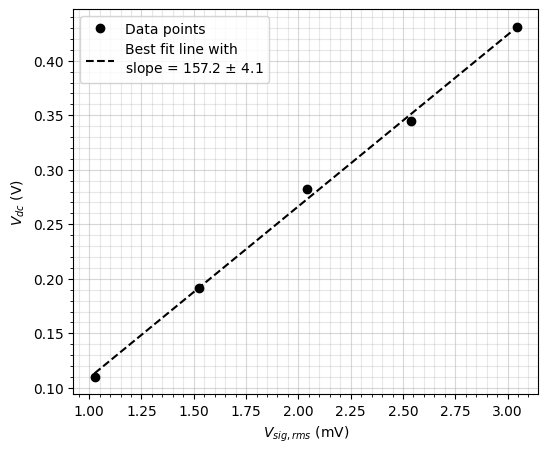
\includegraphics[width=0.9\textwidth]{images/a1.png}
    \caption{300 Hz}
    \end{subfigure}

    \end{figure}
    
    \begin{figure}[H]
    \ContinuedFloat
     
    \bigskip
    \begin{subfigure}{\linewidth}
    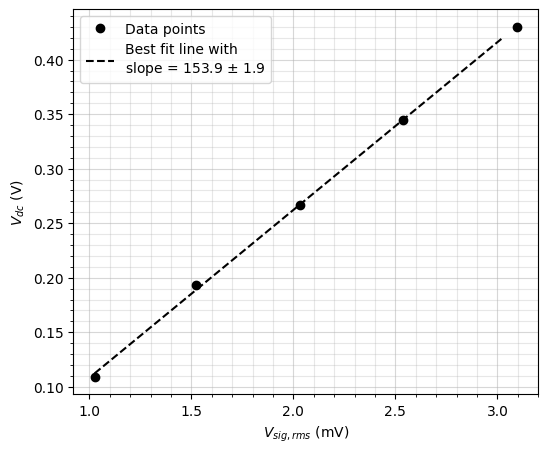
\includegraphics[width=0.95\textwidth]{images/a2.png}
    \caption{600 Hz}
    \end{subfigure}
    
    \bigskip
    \begin{subfigure}{\linewidth}
    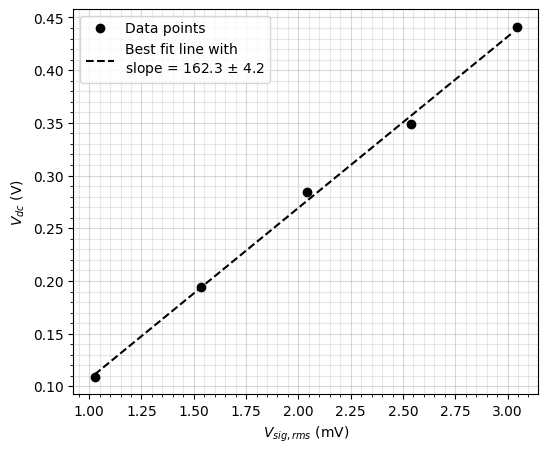
\includegraphics[width=0.95\textwidth]{images/a3.png}
    \caption{900 Hz}
    \end{subfigure}

    \begin{subfigure}{\linewidth}
    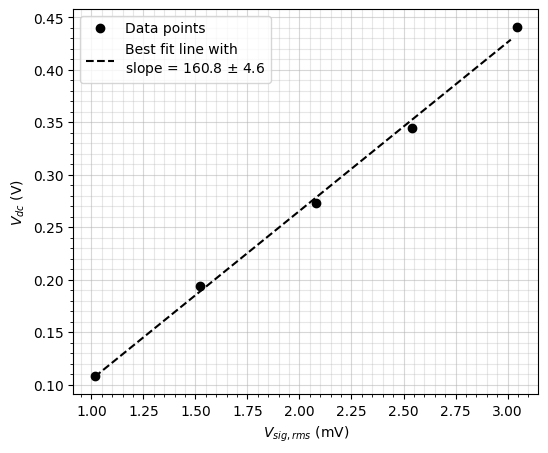
\includegraphics[width=0.9\textwidth]{images/a4.png}
    \caption{1200 Hz}
    \end{subfigure}
    \end{figure}
        
    \begin{figure}[H]
    \ContinuedFloat
    
    % \bigskip
    \begin{subfigure}{\linewidth}
    \centering
    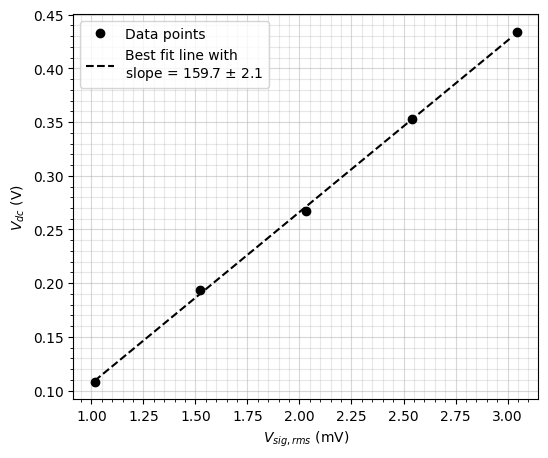
\includegraphics[width=0.80\textwidth]{images/a5.png}
    \caption{1500 Hz}
    \end{subfigure}
    
    \caption{Callibration curve for Gain 50 at different frequencies}
    \label{g1}
\end{figure}

\begin{table}[H]
    \centering
    \begin{tabular}{|c|c|c|} \hline
        $f$ (Hz) &   $\mu$ & Error $(\delta \mu)$ \\\hline
      300 &   157.2 & 4.1 \\
      600 &   153.9 & 1.9 \\
      900 &   162.3 & 4.2 \\
     1200 &   160.8 & 4.6 \\
     1500 &   159.7 & 2.1 \\\hline    
    \end{tabular}
    \caption{$\mu$ and error in $\mu$ for gain 50 from Fig. \ref{g1}. Hence, the average value of $\mu$ for gain 50 is ${ \mu_{50} = 158.8}$.}
\end{table}
% Please add the following required packages to your document preamble:
% \usepackage{multirow}
% \usepackage{graphicx}
\begin{table}[H]
    \centering
    % \resizebox{\columnwidth}{!}{%
    \begin{tabular}{|c|c|c|c|c|}
    \hline
    Frequency& $V_{ac}$ (pp)& $V_{ac, \text{rms}}$& $V_\text{sig, rms}$ & $V_{dc, \text{rms}}$ \\
    (Hz) & (V) & (V) & (V) &  (V) \\ \hline
    \multirow{5}{*}{300} & 1.00 & 0.35355 & 0.00102 & 0.266 \\ \cline{2-5} 
    & 1.50 & 0.53033 & 0.00152 & 0.434 \\ \cline{2-5} 
    & 2.00 & 0.70711 & 0.00203 & 0.572 \\ \cline{2-5} 
    & 2.50 & 0.88388 & 0.00254 & 0.727 \\ \cline{2-5} 
    & 3.00 & 1.06066 & 0.00305 & 0.904 \\ \hline
    \multirow{5}{*}{600} & 1.00 & 0.35355 & 0.00102 & 0.263 \\ \cline{2-5} 
    & 1.50 & 0.53033 & 0.00152 & 0.421 \\ \cline{2-5} 
    & 2.00 & 0.70711 & 0.00203 & 0.572 \\ \cline{2-5} 
    & 2.50 & 0.88388 & 0.00254 & 0.738 \\ \cline{2-5} 
    & 3.00 & 1.06066 & 0.00305 & 0.896 \\ \hline
    \multirow{5}{*}{900} & 1.00 & 0.35355 & 0.00102 & 0.265 \\ \cline{2-5} 
    & 1.50 & 0.53033 & 0.00152 & 0.408 \\ \cline{2-5} 
    & 2.00 & 0.70711 & 0.00203 & 0.578 \\ \cline{2-5} 
    & 2.50 & 0.88388 & 0.00254 & 0.723 \\ \cline{2-5} 
    & 3.00 & 1.06066 & 0.00305 & 0.880 \\ \hline
    \multirow{5}{*}{1200} & 1.00 & 0.35355 & 0.00102 & 0.264 \\ \cline{2-5} 
    & 1.50 & 0.53033 & 0.00152 & 0.429 \\ \cline{2-5} 
    & 2.00 & 0.70711 & 0.00203 & 0.578 \\ \cline{2-5} 
    & 2.50 & 0.88388 & 0.00254 & 0.734 \\ \cline{2-5} 
    & 3.00 & 1.06066 & 0.00305 & 0.901 \\ \hline
    \multirow{5}{*}{1500} & 1.00 & 0.35355 & 0.00102 & 0.264 \\ \cline{2-5} 
    & 1.50 & 0.53033 & 0.00152 & 0.428 \\ \cline{2-5} 
    & 2.00 & 0.70711 & 0.00203 & 0.565 \\ \cline{2-5} 
    & 2.50 & 0.88388 & 0.00254 & 0.717 \\ \cline{2-5} 
    & 3.00 & 1.06066 & 0.00305 & 0.899 \\ \hline
    \end{tabular}%
    % }
    \caption{Data for calibration at gain 100}
    \label{cal100}
    \end{table}

\begin{figure}[H]
    \begin{subfigure}{\linewidth}
    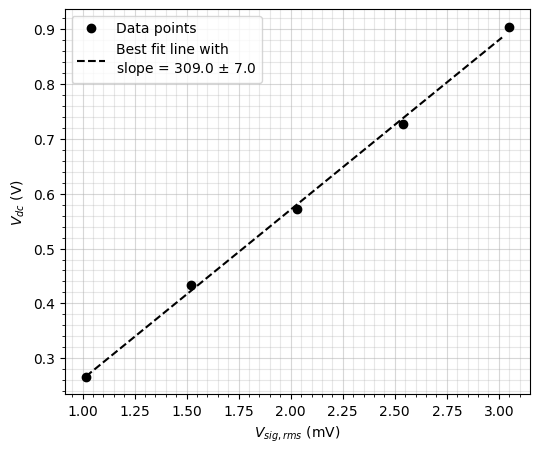
\includegraphics[width=0.9\textwidth]{images/b1.png}
    \caption{300 Hz}
    \end{subfigure}
    
    \bigskip
    \begin{subfigure}{\linewidth}
    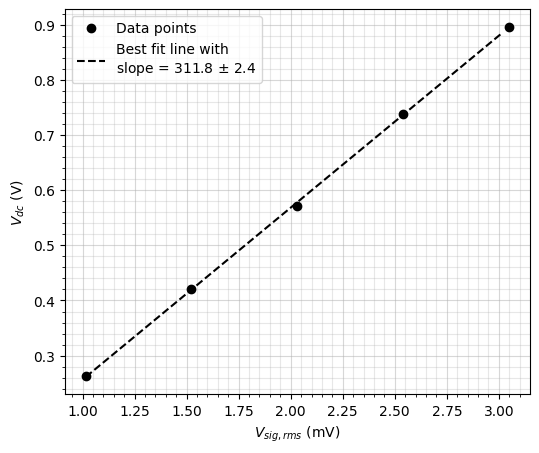
\includegraphics[width=0.9\textwidth]{images/b2.png}
    \caption{600 Hz}
    \end{subfigure}
    
    \bigskip
    \begin{subfigure}{\linewidth}
    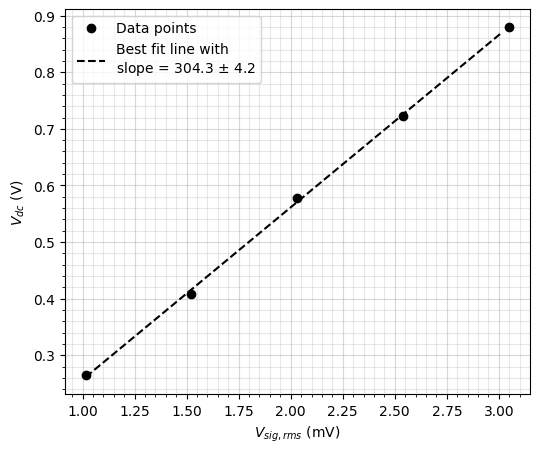
\includegraphics[width=0.9\textwidth]{images/b3.png}
    \caption{900 Hz}
    \end{subfigure}
    \end{figure}
    
    \begin{figure}[H]
    \ContinuedFloat
    \begin{subfigure}{\linewidth}
    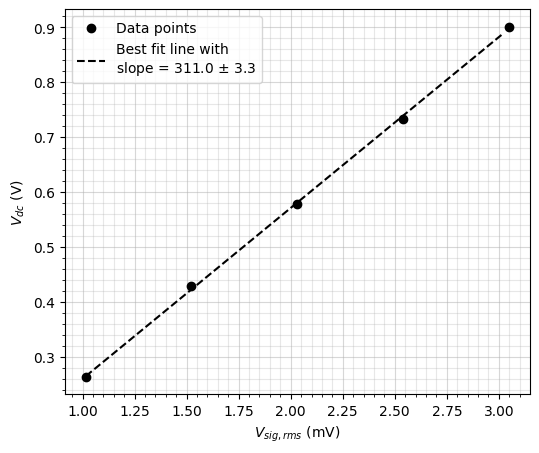
\includegraphics[width=1\textwidth]{images/b4.png}
    \caption{1200 Hz}
    \end{subfigure}
    
    \bigskip
    \begin{subfigure}{\linewidth}
    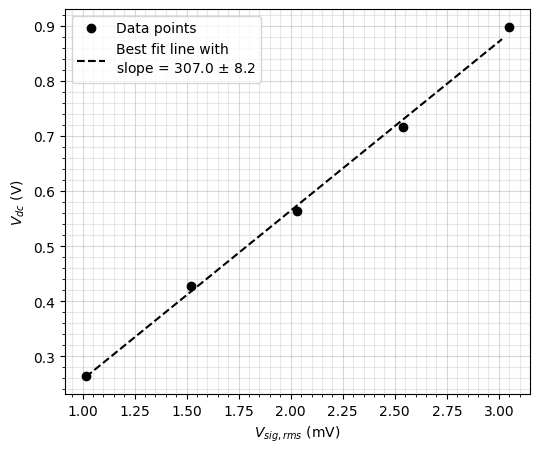
\includegraphics[width=1\textwidth]{images/b5.png}
    \caption{1500 Hz}
    \end{subfigure}
    
    \caption{Callibration curve for Gain 100 at different frequencies}
    \label{g2}
\end{figure}

\begin{table}[H]
    \centering
    \begin{tabular}{|c|c|c|} \hline
        $f$ (Hz) &   $\mu$ & Error $(\delta \mu)$ \\\hline
        300 &   309.0   &              7.0   \\
        600 &   311.8 &              2.4 \\
        900 &   304.3 &              4.2 \\
       1200 &   311.0   &              3.3 \\
       1500 &   307.0   &              8.2 \\ \hline   
    \end{tabular}
    \caption{$\mu$ and error in $\mu$ for gain 100 from Fig. \ref{g2}. Hence, the average value of $\mu$ for gain 100 is ${ \mu_{100} = 308.6}$.}
\end{table}

\subsection{Calculation of Mutual Inductance}

\begin{table}[H]
    \centering
    \begin{tabular}{|c|c|c|c|}
    \hline
    Frequency& $V_{ac}$ (pp)& $V_{ac, \text{rms}}$ & $V_{dc, \text{rms}}$ \\
    (Hz) & (V) & (V)&  (V) \\ \hline
    \multirow{5}{*}{600} & 7.00 & 2.47487 & 0.036 \\ \cline{2-4} 
    & 9.00 & 3.18198 & 0.062 \\ \cline{2-4} 
    & 11.00 & 3.88909 & 0.086 \\ \cline{2-4} 
    & 13.00 & 4.59619 & 0.118 \\ \cline{2-4} 
    & 15.00 & 5.30330 & 0.147 \\ \hline
   \multirow{5}{*}{900} & 7.00 & 2.47487 & 0.072 \\ \cline{2-4} 
    & 9.00 & 3.18198 & 0.094 \\ \cline{2-4} 
    & 11.00 & 3.88909 & 0.141 \\ \cline{2-4} 
    & 13.05 & 4.61387 & 0.184 \\ \cline{2-4} 
    & 15.00 & 5.30330 & 0.223 \\ \hline
   \multirow{5}{*}{1200} & 7.05 & 2.49255 & 0.126 \\ \cline{2-4} 
    & 9.00 & 3.18198 & 0.158 \\ \cline{2-4} 
    & 11.00 & 3.88909 & 0.229 \\ \cline{2-4} 
    & 13.00 & 4.59619 & 0.285 \\ \cline{2-4} 
    & 15.00 & 5.30330 & 0.344 \\ \hline
   \multirow{5}{*}{1500} & 7.00 & 2.47487 & 0.154 \\ \cline{2-4} 
    & 9.00 & 3.18198 & 0.233 \\ \cline{2-4} 
    & 11.00 & 3.88909 & 0.299 \\ \cline{2-4} 
    & 13.00 & 4.59619 & 0.364 \\ \cline{2-4} 
    & 15.00 & 5.30330 & 0.439 \\ \hline
    \end{tabular}%
    \caption{Data for calculation of Mutual Induction at 100 gain}
    \label{mutual}
    \end{table}

\begin{figure}[H]
    \centering
    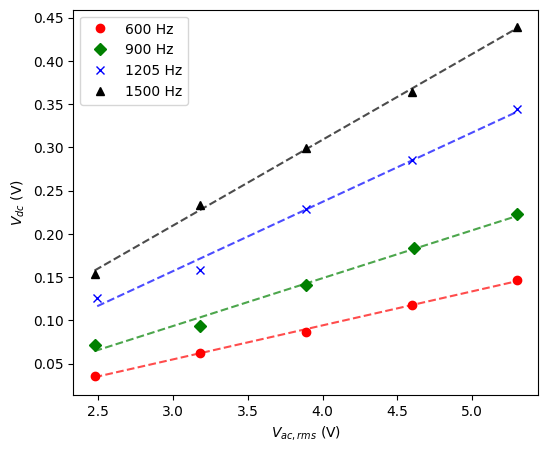
\includegraphics[width=1\columnwidth]{images/e1.png}
    \caption{$V_{dc}$ vs $V_{ac}$ at different frequencies for measurement of mutual induction at gain 100}
    \label{g3}
\end{figure}

Now the slope of the graph in Fig. \ref{g4}, $\beta=6.8 \times 10^{-5}$ Hz$^{-1}$ is given by Eq. 10. Substituting the value with $R=4.8$ k$\Omega$,
\begin{align*}
    M = \frac{\beta R}{2 \pi \mu_{100}} = 168.3\,\mu\text{H}
\end{align*}

\begin{figure}[H]
    \centering
    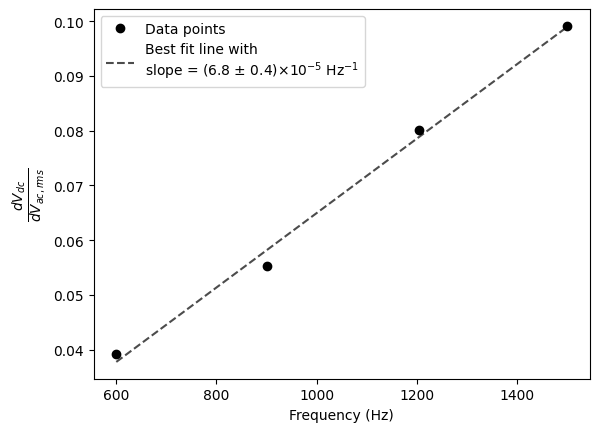
\includegraphics[width=0.9\columnwidth]{images/e2.png}
    \caption{$\frac{dV_{dc}}{dV_{ac}}$ vs frequency plot to calculate Mutual Inductance}
    \label{g4}
\end{figure}

\subsection{Measurement of Low Resistance}

The value of Low resistance is given by

\begin{align*}
    \text{slope }&=\frac{dV_{dc}}{dV_{ac}}=\frac{\mu r}{R}\\
    \text{where }\frac{1}{R} &= \frac{1}{0.995} + \frac{1}{0.995}
\end{align*}

Hence, $R=0.498$ kHz.

\begin{table}[H]
    \centering
    \begin{tabular}{|c|c|c|c|}
    \hline
    Frequency& $V_{ac}$ (pp)& $V_{ac, \text{rms}}$ & $V_{dc, \text{rms}}$ \\
    (Hz) & (V) & (V)&  (V) \\ \hline
    \multirow{5}{*}{300} & 1.00 & 0.35355 & -0.004 \\ \cline{2-4} 
 & 1.50 & 0.53033 & 0.020 \\ \cline{2-4} 
 & 2.00 & 0.70711 & 0.043 \\ \cline{2-4} 
 & 2.50 & 0.88388 & 0.054 \\ \cline{2-4} 
 & 3.00 & 1.06066 & 0.076 \\ \hline
\multirow{5}{*}{600} & 1.00 & 0.35355 & -0.006 \\ \cline{2-4} 
 & 1.50 & 0.53033 & 0.017 \\ \cline{2-4} 
 & 2.00 & 0.70711 & 0.035 \\ \cline{2-4} 
 & 2.50 & 0.88388 & 0.058 \\ \cline{2-4} 
 & 3.00 & 1.06066 & 0.085 \\ \hline
\multirow{5}{*}{900} & 1.00 & 0.35355 & -0.006 \\ \cline{2-4} 
 & 1.50 & 0.53033 & 0.017 \\ \cline{2-4} 
 & 2.00 & 0.70711 & 0.042 \\ \cline{2-4} 
 & 2.50 & 0.88388 & 0.058 \\ \cline{2-4} 
 & 3.00 & 1.06066 & 0.084 \\ \hline
\multirow{5}{*}{1200} & 1.00 & 0.35355 & -0.007 \\ \cline{2-4} 
 & 1.50 & 0.53033 & 0.017 \\ \cline{2-4} 
 & 2.00 & 0.70711 & 0.035 \\ \cline{2-4} 
 & 2.50 & 0.88388 & 0.058 \\ \cline{2-4} 
 & 3.00 & 1.06066 & 0.083 \\ \hline
\multirow{5}{*}{1500} & 1.00 & 0.35355 & -0.001 \\ \cline{2-4} 
 & 1.50 & 0.53033 & 0.016 \\ \cline{2-4} 
 & 2.00 & 0.70711 & 0.043 \\ \cline{2-4} 
 & 2.50 & 0.88388 & 0.057 \\ \cline{2-4} 
 & 3.00 & 1.06066 & 0.083 \\ \hline
    \end{tabular}%
    \caption{Data for measurement of Low resistance at
    50 gain}
    \label{res50}
    \end{table}

\begin{figure}[H]
    \begin{subfigure}{\linewidth}
    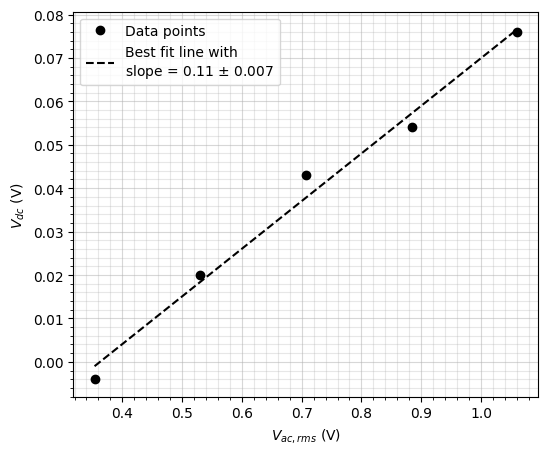
\includegraphics[width=1\textwidth]{images/c1.png}
    \caption{300 Hz}
    \end{subfigure}
    
    % \bigskip
    \begin{subfigure}{\linewidth}
    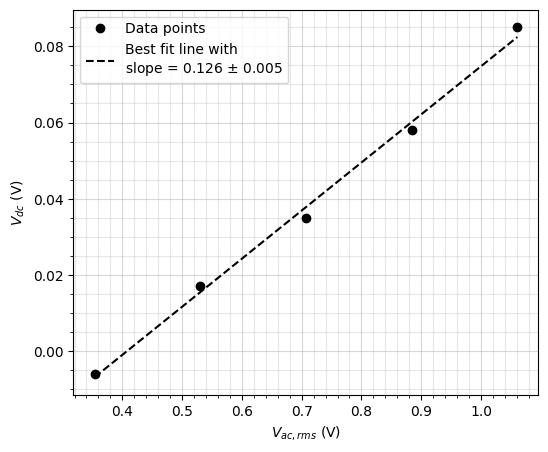
\includegraphics[width=1\textwidth]{images/c2.png}
    \caption{600 Hz}
    \end{subfigure} 
    \bigskip
    \begin{subfigure}{\linewidth}
    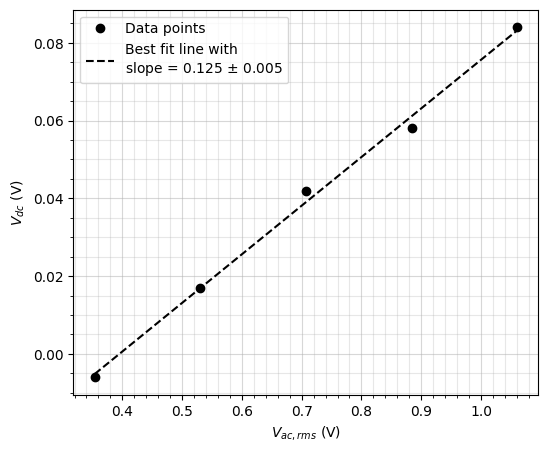
\includegraphics[width=\textwidth]{images/c3.png}
    \caption{900 Hz}
    \end{subfigure}
   
    \end{figure}
    
    \begin{figure}[H]
    \ContinuedFloat
    \begin{subfigure}{\linewidth}
    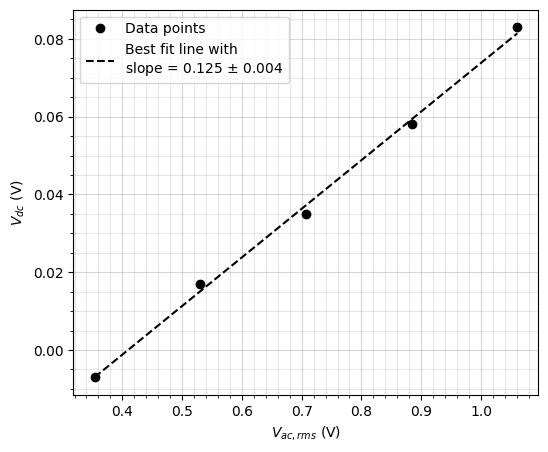
\includegraphics[width=1\textwidth]{images/c4.png}
    \caption{1200 Hz}
    \end{subfigure}
    
    \bigskip
    \begin{subfigure}{\linewidth}
    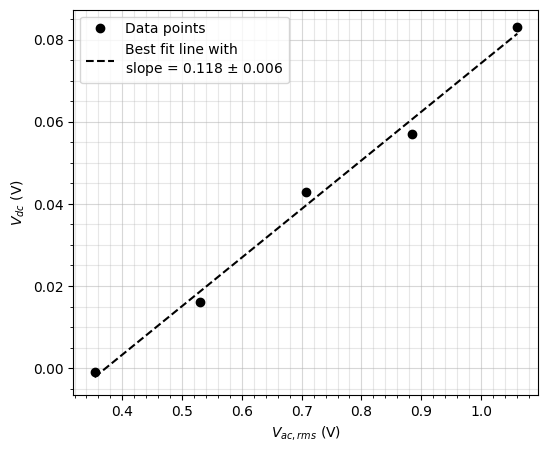
\includegraphics[width=1\textwidth]{images/c5.png}
    \caption{1500 Hz}
    \end{subfigure}
    
    \caption{$V_{ac}$ vs $V_{dc}$ plots for Gain 50 at different frequencies for measurement of low resistance}
\end{figure}

\begin{table}[H]
    \centering
    \begin{tabular}{|c|c|c|c|c|} \hline
        $f$ & slope & Error in  & $r$ & $\delta r$ \\
        (Hz) & & slope & ($\Omega$) & ($\Omega$) \\\hline
        300 & 0.110 & 0.007 & 0.344 &        0.023 \\
        600 & 0.126 & 0.005 & 0.395 &        0.016 \\
        900 & 0.125 & 0.005 & 0.392 &        0.015 \\
        1200 & 0.125 & 0.004 & 0.392 &        0.012 \\
        1500 & 0.118 & 0.006 & 0.370 &        0.020 \\\hline
    \end{tabular}
    \caption{The slopes of plots from Fig. 7 and the calculated $r$ values (using Eq. 14) and their corresponding error values (using Eqn. 17)}
\end{table}

Thus the average value of $r$ obtained here is $r_{50}=0.382\,\Omega$.

\begin{table}[H]
    \centering
    \resizebox{0.5\columnwidth}{!}{%
    \begin{tabular}{|c|c|c|c|}
    \hline
    Frequency& $V_{ac}$ (pp)& $V_{ac, \text{rms}}$ & $V_{dc, \text{rms}}$ \\
    (Hz) & (V) & (V)&  (V) \\ \hline
    \multirow{5}{*}{300} & 1.00 & 0.35355 & 0.015 \\ \cline{2-4} 
 & 1.50 & 0.53033 & 0.052 \\ \cline{2-4} 
 & 2.00 & 0.70711 & 0.089 \\ \cline{2-4} 
 & 2.50 & 0.88388 & 0.139 \\ \cline{2-4} 
 & 3.00 & 1.06066 & 0.182 \\ \hline
\multirow{5}{*}{600} & 1.00 & 0.35355 & 0.036 \\ \cline{2-4} 
 & 1.50 & 0.53033 & 0.083 \\ \cline{2-4} 
 & 2.00 & 0.70711 & 0.129 \\ \cline{2-4} 
 & 2.50 & 0.88388 & 0.168 \\ \cline{2-4} 
 & 3.00 & 1.06066 & 0.182 \\ \hline
\multirow{5}{*}{900} & 1.00 & 0.35355 & 0.033 \\ \cline{2-4} 
 & 1.50 & 0.53033 & 0.078 \\ \cline{2-4} 
 & 2.00 & 0.70711 & 0.126 \\ \cline{2-4} 
 & 2.50 & 0.88388 & 0.164 \\ \cline{2-4} 
 & 3.00 & 1.06066 & 0.211 \\ \hline
\multirow{5}{*}{1200} & 1.00 & 0.35355 & 0.035 \\ \cline{2-4} 
 & 1.50 & 0.53033 & 0.081 \\ \cline{2-4} 
 & 2.00 & 0.70711 & 0.119 \\ \cline{2-4} 
 & 2.50 & 0.88388 & 0.163 \\ \cline{2-4} 
 & 3.00 & 1.06066 & 0.205 \\ \hline
\multirow{5}{*}{1500} & 1.00 & 0.35355 & 0.034 \\ \cline{2-4} 
 & 1.50 & 0.53033 & 0.078 \\ \cline{2-4} 
 & 2.00 & 0.70711 & 0.122 \\ \cline{2-4} 
 & 2.50 & 0.88388 & 0.160 \\ \cline{2-4} 
 & 3.00 & 1.06066 & 0.209 \\ \hline
    \end{tabular}%
    }
    \caption{Data for measurement of Low resistance at
    100 gain}
    \label{res100}
    \end{table}

\begin{figure}[H]
    \begin{subfigure}{\linewidth}
    \centering
    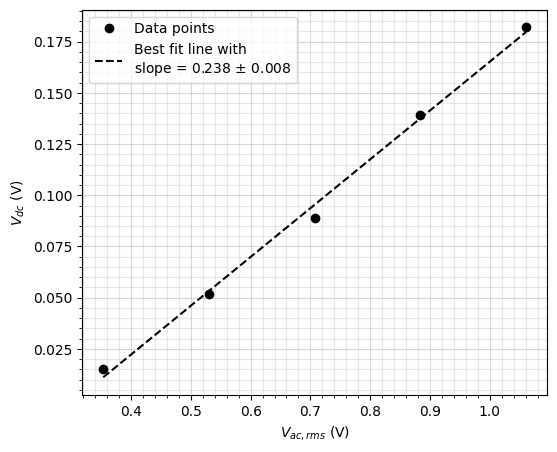
\includegraphics[width=0.8\textwidth]{images/d1.png}
    \caption{300 Hz}
    \end{subfigure}
    
    \begin{subfigure}{\linewidth}
    \centering
    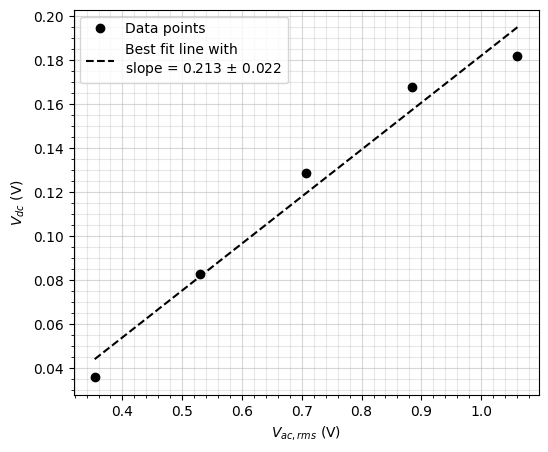
\includegraphics[width=0.8\textwidth]{images/d2.png}
    \caption{600 Hz}
    \end{subfigure} 
     
    \end{figure}
    
    \begin{figure}[H]
    \ContinuedFloat
     % \bigskip
    % \begin{subfigure}{\linewidth}
    % 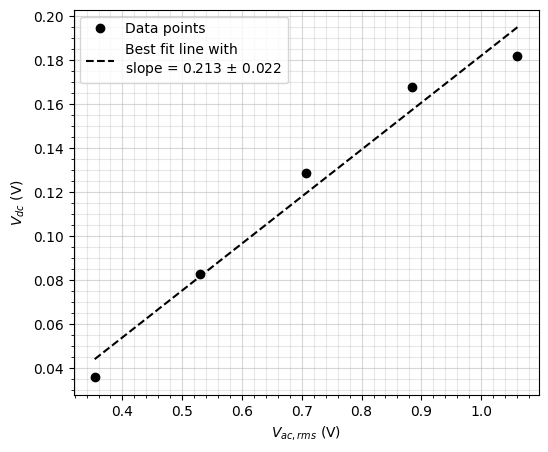
\includegraphics[width=0.95\textwidth]{images/d2.png}
    % \caption{600 Hz}
    % \end{subfigure} 
    % \bigskip
    \begin{subfigure}{\linewidth}
    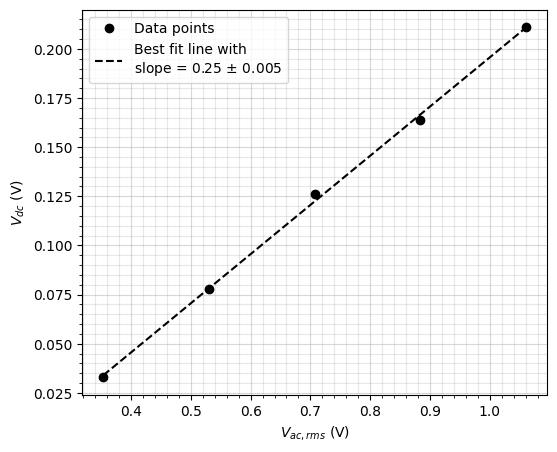
\includegraphics[width=0.9\textwidth]{images/d3.png}
    \caption{900 Hz}
    \end{subfigure}
    % \bigskip

    \begin{subfigure}{\linewidth}
    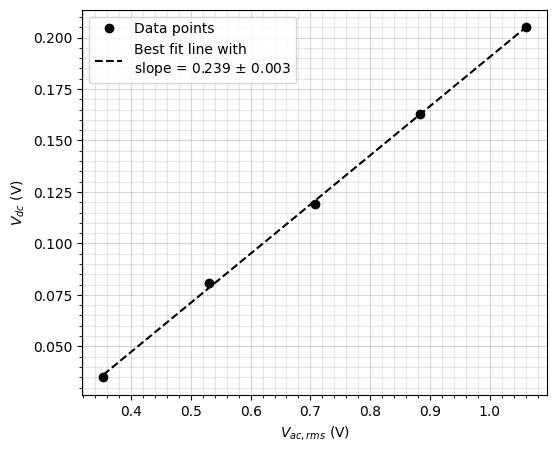
\includegraphics[width=0.9\textwidth]{images/d4.png}
    \caption{1200 Hz}
    \end{subfigure}
    
    \end{figure}
        
    \begin{figure}[H]
    \ContinuedFloat
    % \bigskip
    \begin{subfigure}{\linewidth}
    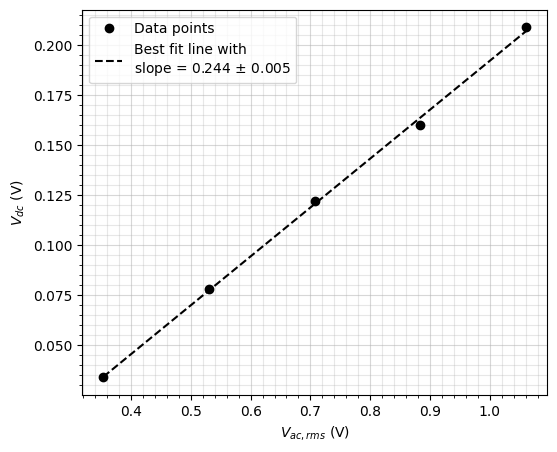
\includegraphics[width=0.9\textwidth]{images/d5.png}
    \caption{1500 Hz}
    \end{subfigure}
    
    \caption{$V_{ac}$ vs $V_{dc}$ plots for Gain 100 at different frequencies for measurement of low resistance}
\end{figure}

\begin{table}[H]
    \centering
    \begin{tabular}{|c|c|c|c|c|} \hline
        $f$ & slope & Error in  & $r$ & $\delta r$ \\
        (Hz) & & slope & ($\Omega$) & ($\Omega$) \\\hline
        300 & 0.238 & 0.008 & 0.384 &        0.015 \\
        600 & 0.213 & 0.022 & 0.344 &        0.035 \\
        900 & 0.250 & 0.005 & 0.403 &        0.010 \\
        1200 & 0.239 & 0.003 & 0.385 &        0.009 \\
        1500 & 0.244 & 0.005 & 0.394 &        0.010 \\\hline
    \end{tabular}
    \caption{The slopes of plots from Fig. 8 and the calculated $r$ values (using Eq. 14) and their corresponding error values (using Eqn. 17)}
\end{table}

Thus the average value of $r$ obtained here is $r_{100}=0.379\,\Omega$.
Hence the final average value comes out to be,

\begin{align*}
    r = \frac{r_{50}+r_{100}}{2} = 0.380\,\Omega
\end{align*}

\section{Error Analysis}

The calibration error is the error in the slope which
is given in tables II and IV. The error in mutual inductance is given by,

\begin{align}
    \delta M = M\sqrt{\left(\frac{\delta\mu}{\mu}\right)^2 + \left(\frac{\delta\beta}{\beta}\right)^2 + \left(\frac{\delta R}{ R}\right)^2}
\end{align}

where

\begin{align}
    \delta \mu = \frac{1}{\sqrt{5}}\sqrt{\sum_{f_i}\left(\mu_{f_i}\right)^2}
\end{align}

for each of the 5 values of $f_i$ in tables II and IV. This comes out to be,

\begin{itemize}
    \item For gain 50, $\delta \mu_{50} = 3.6$
    \item For gain 100, $\delta \mu_{100} = 5.5$\\
\end{itemize}

Now using $\delta \mu_{100} = 5.5$, $\delta \beta = 0.4 \times 10^{-5}$ Hz$^{-1}$ (from Fig. 6) and $\delta R = 0.01$ k$\Omega$, we get $\delta M = 9.5\,\mu$H.

For the error in $r$, we get
\begin{align}
    \delta r_{f_i} = r_{f_i}\sqrt{\left(\frac{\delta\mu}{\mu}\right)^2 + \left(\frac{\delta\,\text{slope}}{\text{slope}}\right)^2 + \left(\frac{\delta R}{ R}\right)^2}
\end{align}

Tables VII and IX show the $\delta r$ for every value of $r$ calculated using Eq. 17.
The average error in $r$ can be calculated as,

\begin{align}
    \delta r = \frac{1}{\sqrt{5}}\sqrt{\sum_{f_i}\left(r_{f_i}\right)^2}
\end{align}
for each of the 5 values of $f_i$ in. Using this the errors are $\delta r_{50} = 0.018\,\Omega$ and $\delta r_{100} = 0.019\,\Omega$ for both values of gain. Thus,

% \begin{itemize}
%     \item For gain 50, $\delta r_{50} = 0.018\,\Omega$
%     \item For gain 100, $\delta r_{100} = 0.019\,\Omega$\\
% \end{itemize}

% We can also take the mean error from both the measurements as,

\begin{align*}
    \delta r &= \frac{1}{\sqrt{2}}\sqrt{\left(0.018\right)^2+\left(0.019\right)^2}= 0.018\,\Omega
\end{align*}